\chapter{Analysis}

\section{Datasets}
This study employs two distinct datasets to construct a feature table for use in classification algorithms. Both datasets are the result of Monte Carlo simulations conducted via the SNiPER software \cite{sniper}.

\subsection*{IBD Dataset}
The primary dataset, known as the IBD dataset, is specifically designed for analyzing potential Inverse Beta Decay events, assuming that the sources of antineutrinos are the reactors (Table \ref{tab:IBD_reactor_source}) providing a combined output of 57.4 events/day. Importantly, the dataset does not contain any contribution from background events.

The IBD dataset has the following key features:

\begin{small}
\begin{itemize}
	\item \texttt{SimID}: a unique identifier for each true IBD pair. A prompt-delayed pair originating from an IBD event will share the same SimID.
	\item \texttt{(x, y, z)}: the reconstructed coordinates of the point within the detector where the IBD event occurred.
	\item \texttt{E}: the energy of the individual event as recorded by the detector.
	\item \texttt{t}: the timestamp of when the event occurred.
\end{itemize}
\end{small}

Upon completion of the comprehensive simulation, which incorporates the modeling of the trigger system to accurately reflect its efficiency, the resulting dataset has a total of 2,977,856 events

\subsection*{BKG Dataset}
The second dataset is exclusively composed of events related to radioactivity. 
The file structure of the BKG dataset remains identical to that of the IBD dataset. However, due to the uncorrelated nature of events in the BKG dataset, a unique SimID is assigned to each event, ensuring its distinctiveness from all other events. 

In Table \ref{tab:BKG_gen} are shown rates that are used as inputs for the simulation process.

\begin{table}[htp]
	\begin{minipage}[t]{0.45\linewidth}
		\centering
		\small
		\begin{tabular}{cc}
			\toprule
			\textbf{Dataset Name} & \textbf{Rates} \\
			\midrule
			U238@LS  & 3.234 Hz \\
			Th232@LS & 0.733 Hz \\
			K40@LS  & 0.53 Hz \\
			Pb210@LS  & 17.04 Hz \\
			C14@LS  & $3.3 \cdot 10^{4}$ Hz \\
			Kr85@LS  & 1.163 Hz \\
			U238@Acrylic  & 98.41 Hz \\
			Th232@Acrylic  & 22.29 Hz \\
			K40@Acrylic  & 161.25 Hz \\
			\bottomrule
		\end{tabular}
	\end{minipage}
\hspace{0.5cm}
	\begin{minipage}[t]{0.45\linewidth}
		\centering
		\small
		\begin{tabular}{cc}
			\toprule
			\textbf{Dataset Name} & \textbf{Rates}  \\
			\midrule
			U238@node/bar  & 2102.36 Hz \\
			Th232@node/bar  & 1428.57 Hz \\
			K40@node/bar  & 344.5 Hz \\
			Co60@node/bar  & 97.5 Hz \\
			U238@PMTGlass  & $4.90 \cdot  10^{6}$ Hz \\
			Th232@PMTGlass  & $8.64 \cdot  10^{5}$ Hz \\
			K40@PMTGlass  & $4.44 \cdot  10^{5}$ Hz \\
			Tl208@PMTGlass  & $1.39 \cdot  10^{5}$ Hz \\
			Rn222@WaterRadon  & 90 Hz \\
			\bottomrule
		\end{tabular}
	\end{minipage}
	\caption{Table of isotopes, and rates used as simulation inputs}
	\label{tab:BKG_gen}
\end{table}

This background represents all the contributions from radioactive decays $(\alpha, \beta, \gamma)$ both internal and external to the detector, but that have deposited energy inside the detector.

The rates provided in the Table \ref{tab:BKG_gen} serve as assumptions regarding the occurrence of events from different isotopes and their respective decay rates. However, it is important to consider that the actual event rate in the dataset is influenced by various factors, including trigger thresholds, event multiplicity, energy deposition location, which may extend beyond the detector, and experimental conditions. As a result, the observed event rate in the final dataset deviate from the initially assumed rates.


It is important to underline the differences in the location of the isotopes in the detector:
\begin{small} 
\begin{itemize}
	\item \textbf{Liquid Scintillator (LS):} The main part of the detector, where isotopes U238, Th232, K40, Pb210, C14, and Kr85 are found. It's worth noting that C14 contributes with a high decay rate of 33 kHz.
	\item \textbf{Acrylic:} This constitutes the detector walls, hosting isotopes U238, Th232, and K40.
	\item \textbf{Node/bar:} This is the metallic structure supporting the detector. Here, isotopes U238, Th232, K40, and Co60 are located.
	\item \textbf{PMT Glass:} The glass of the photomultipliers containing isotopes U238, Th232, K40, and Tl208. The isotope U238 stands out with an extremely high decay rate of 4.9 MHz.
	\item \textbf{WaterRadon:} This represents the gas present in the water surrounding the detector and inside the detector during the initial filling stages.
\end{itemize}
\end{small}

However, not all generated - and listed in the table - events interact with the detector. Some events are so low in energy that they aren't sufficient to produce a signal in the photomultiplier tubes (PMTs) and, therefore, to trigger the acquisition of the event. Despite these caveats, the table offers a valuable understanding of the decay contributions within the detector's different components.

It is important to note that U238@PMTGlass has one of the highest decay rates, at approximately 4.90 MHz. This high rate indicates that Uranium-238 within the PMT Glass is highly active and undergoes decay at a very rapid pace. 
Similarly, Th232@PMTGlass also exhibits a high decay rate, around 864 kHz. Like U-238, Th-232 in the PMT Glass is highly active. Such high activity  will contribute substantially to the background within the detector.


The dataset is made of comprises a total of 8,841,188 recorded events, obtained from a one-day exposure.
%TODO-> Mention unbalanced datasets problem

\newpage

\section{Feature creation}
The process of feature engineering plays a pivotal role in the successful development of models for detecting IBD events. It is a critical step where the majority of the model's performance is determined. This crucial process involves loading the two distinct datasets mentioned earlier: one for IBD events and the other for radioactivity background.


\subsection{IBD Features Table}
As we mentioned earlier, an IBD event is characterized by two correlated signals with different energies, positions, and times. 

To create the feature table, all possible pairs of events within the dataset were considered, without repetition. The ascending temporal order in which the features are created is crucial in feature determination, considering that neutron capture occurs temporally subsequent to electron-positron annihilation. 
Given a pair $i-j$ in the IBD dataset, the following features were constructed:


\begin{itemize}
	 
	\item $\mathbf{R_{prompt}}$: This feature represents the distance of the prompt signal, calculated as the distance from the origin to the point $(x_i, y_i, z_i)$ in the detector space where the prompt signal occurred.	
	
	\item $\mathbf{R_{delayed}}$: Similar to $R_{prompt}$, this feature represents the distance of the delayed signal, calculated as the distance from the origin to the point $(x_j, y_j, z_j)$ in the detector space where the delayed signal occurred.

	\item $\mathbf{E_{prompt}}$: This feature represents the energy of the prompt signal. It is the characteristic energy released during ionization and subsequent annihilation of a positron with an electron in the scintillator liquid.

	\item $\mathbf{E_{delayed}}$: This feature represents the energy of the delayed signal. It is the energy released when a neutron is captured by the scintillator liquid.

	\item $\mathbf{\Delta t}$: This feature represents the time difference between the two events. It captures the temporal delay between the occurrence of the prompt and delayed signals.

	\item $\mathbf{\Delta R}$: This feature represents the spatial distance between the two events. It captures the spatial separation between the points in the detector space where the prompt and delayed signals occurred.

\begin{equation*}
  \Delta R = \sqrt{{(x_i - x_j)^2 + (y_i - y_i)^2 + (z_i - z_j)^2}}) 
\end{equation*}


\end{itemize}
These features encapsulate the temporal and spatial differences between the prompt and delayed signals, as well as their respective energies, providing a comprehensive representation of the unique characteristics of IBD events.


\subsubsection*{Event Labeling}
The labeling system is based on the SimID. An event pair is assigned a label of 1 if it represents a true IBD event generated as part of the same simulation. On the other hand, a label of 0 indicates uncorrelated background events that originate from different simulations.
For the radioactivity dataset, the feature calculation was performed in a manner analogous to the IBD dataset. The key difference is that event pairs from the radioactivity dataset are labeled as BKG events, hence assigned a label of 0.

\subsubsection*{Efficient Feature Calculation}
To enhance computational speed due to the large dataset size and the complexity of feature calculation, a parallel computing approach was implemented. The calculations were carried out on a virtual machine hosted on Cloud Veneto, which had 14 CPU cores available. The feature calculation task was divided into multiple sub-tasks, allowing them to be executed simultaneously by different CPU cores. This parallelization strategy significantly decreased the overall computation time required for the task.

To further optimize the computation, a method was implemented to only consider event pairs where the delayed event occurs within a time window of $5*\tau$ from the prompt event. This approach is based on the fact that the time delay between the prompt and delayed events in Inverse Beta Decay typically follows an exponential distribution, a characteristic of radioactive decay processes. While this method significantly reduces the number of potential event pairs, it might exclude only about $0.7\%$ of IBD events that occur outside this time window, but this trade-off is deemed acceptable.

The distribution of the features are presented in the plots of Figure \ref{fig:hist_features}.


\begin{figure}[h!]
	\centering
	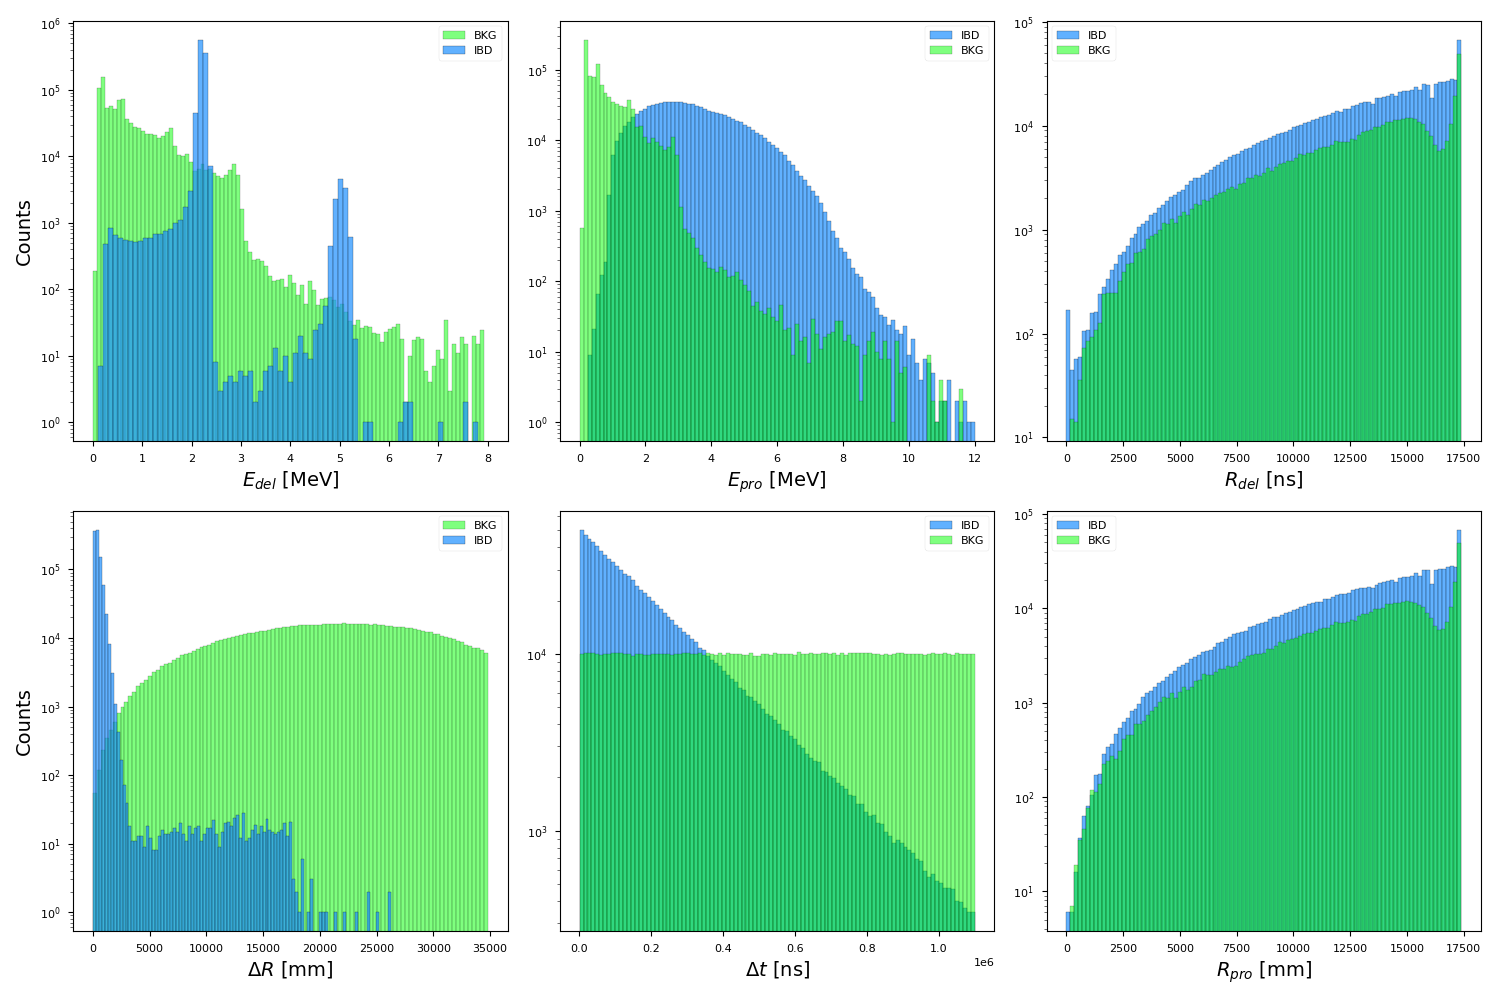
\includegraphics[width=0.9\linewidth]{Images/hist_features.png}
	\caption{Features histograms}
	\label{fig:hist_features}
\end{figure}



\subsubsection*{Feature distribution}
In the graph of Figure \ref{fig:hist_features}, focusing only on IBD events, it is clearly observable for $E_{del}$ feature, the distinct characteristics of the IBD events, such as the peaks at $2.2 MeV$ and $4.9 MeV$, and the clearly visible positron spectrum in the $E_{pro}$ feature. The distribution of $R_{del}$ and $R_{prompt}$ follows the expected pattern for events that are uniformly distributed within the detector. This distribution aligns with the spherical shape of the detector, where IBD events are more likely to occur in the outer region due to the greater volume of liquid scintillator in that area. The observed distribution adheres to the expected $R^3$ distribution characteristic of uniformly distributed events within a spherical detector.

Additionally, the plot for \( \Delta R \) clearly shows that IBD events are generally very close to each other, with a peak observed for \( \Delta R < 3000 \) mm. The \( \Delta t \) distribution for IBD events follows a decreasing exponential distribution, which appears as a straight line since the plot is logarithmic on the y-axis.

For the BKG events, on the other hand, we can see that they have a fundamentally different distribution for \( \Delta R \) compared to IBD events. There is a higher occurrence of events with \( \Delta R > 3000 \) mm, and even at \( \Delta R \approx 35000 \) mm, which corresponds to events occurring in opposite parts of the detector, are significantly probable, as expected for accidental coincidences. This allows to distinguish IBD events from BKG events. For the \( \Delta t \) distribution of BKG events, it is observed to be nearly constant across all possible \( \Delta t \) values. As the energy \( E_{del} \) increases, the number of \( E_{del} \) events decreases. Despite the presence of well-defined peaks in the data, these peaks do not correspond to the expected peaks from neutron capture.

Another notable characteristic is the remarkable similarity between the spectra of the prompt and delayed signals, providing evidence that they arise from accidental coincidences.

\( R_{del} \) and \( R_{prompt} \) for BKG events show a distribution similar to IBD events, with the distinction that there are more counts in the final part of the detector, where there is a higher presence of BKG events. This is due to, as evident from the Table \ref{tab:BKG_gen}, the acrylic, steel bars, PMT glass, and the presence of radon in the water.

Upon inspection, a noticeable decline around the $R \approx 16500$ mm range is evident in the distribution of both \(R_{\text{del}}\) and \(R_{\text{pro}}\). This can be largely attributed to C14, a low-energy decay isotope. Its presence leads to more detections at the detector's center than the edge due to its relatively low energy release, which barely meets the threshold for activating the necessary PMTs, in the outer regions of the detector, where the collection of scintillation light is less efficient.

\section{Models}
This chapter introduces several algorithms, starting with a manual cut-based approach, \textbf{Manual Cut}, which sets criteria based on event physics and background noise. Manual Cut is considered the current state-of-the-art method and serves as the benchmark against which other methods are compared. Additionally, machine learning-based algorithms, specifically \textbf{Boosted Decision Trees} and \textbf{Neural Networks}, are discussed. 

\subsubsection{Dataset pre-processing}
The dataset used for model evaluation was pre-processed by combining the feature tables for IBD and BKG events in a random manner. To address class imbalance, surplus BKG event pairs were removed.

The dataset was divided into three subsets: training, validation, and test datasets. The training dataset, which accounted for $80\%$ of the original dataset, was used for model training. The test dataset, constituting $20\%$ of the original dataset, provided an independent evaluation of the final models. Additionally, a validation dataset was created, representing $10\%$ of the training set, and it allowed for performance evaluation during the training process.

By following this methodology, we ensured reliable comparisons and drew meaningful conclusions from the evaluation of the models.

\subsection{Manual Cut}
The algorithm is designed to suppress various types of background while maintaining high efficiency for IBD events. The selection criteria, or "\textbf{cuts}" are implemented using Python, and are applied to the Features Tables discussed above. Each cut within the algorithm serves a distinct purpose in the overall event selection process. It is essential to emphasize that the selection criteria for the cuts have been employed as outlined in the referenced paper \cite{Sub_osci}.

The key components of the event selection algorithm are as follows:

\begin{enumerate}
	\item \textbf{Delta Time ($\Delta t$) and Delta Radius ($\Delta R$) cuts}: The first cut is applied on the time delay (Figure \ref{fig:delta_t_cut}) and the radial distance (Figure \ref{fig:delta_radius_cut}) between the prompt and delayed signals. The criteria are:
	\begin{itemize}
		\item Time separation between the prompt and delayed signals should be less than 1.0 ms.
		\item Spatial 3D separation should be less than 1.5 m.
	\end{itemize}

	The cut values for Delta Time (\(\Delta t\)) and Delta Radius (\(\Delta R\)) are empirically set based on Inverse Beta Decay events.The 1.0 ms time cut is determined based on the characteristic time scale of neutron thermalization and capture, denoted as $\tau$. This characteristic time scale represents the average time it takes for a neutron to undergo thermalization and subsequently get captured, while the 1.5 m spatial cut considers the short distance neutrons typically travel before capture.

\begin{figure}[h!]
	\centering
	\begin{minipage}{0.5\textwidth}
		\centering
		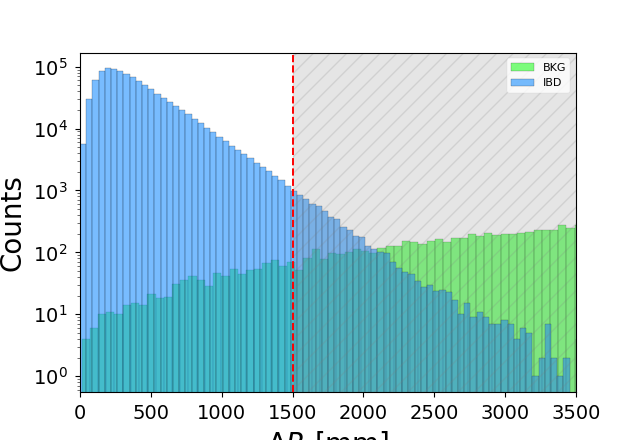
\includegraphics[width=7cm]{Images/Cut/delta_radius.png}
		\caption{$\Delta R$ cut}
		\label{fig:delta_radius_cut}
	\end{minipage}%
	\begin{minipage}{0.5\textwidth}
		\centering
		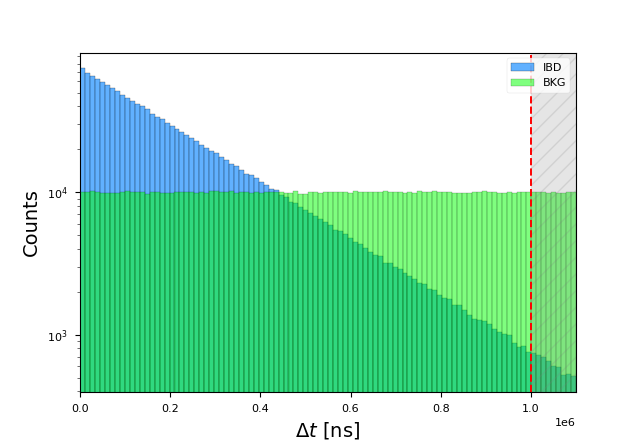
\includegraphics[width=7cm]{Images/Cut/delta_time.png}
		\caption{$\Delta t$ cut}
		\label{fig:delta_t_cut}
	\end{minipage}
\end{figure}


	\vspace{-1\baselineskip}

	\item \textbf{Energy of the Prompt Signal ($E_{pro}$) Cut}: The next cut is applied on the energy of the prompt signal (Figure \ref{fig:e_pto_cut}), which is the initial signal produced by the antineutrino interaction. The criteria are:
	\begin{itemize}
		\item Energy of the prompt signal should be within the [0.7, 12.0] MeV range.
	\end{itemize}
	
	\begin{adjustbox}{minipage={\linewidth}, valign=t}
		
		\begin{wrapfigure}{t}{0.5\linewidth}
			
			\vspace{-1\baselineskip}
			\caption{$E_{pro}$ cut}
			\vspace{-0.5\baselineskip}
			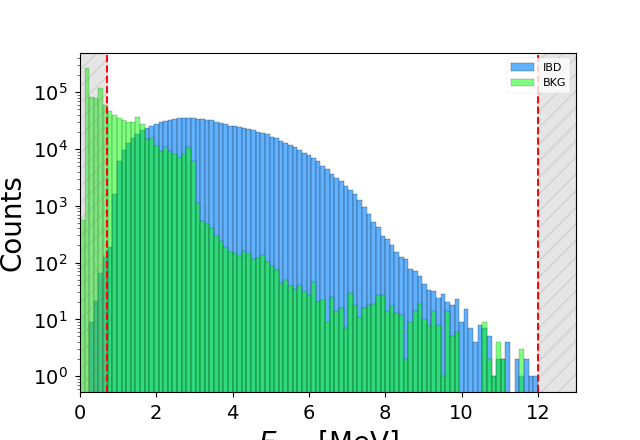
\includegraphics[width=7.5cm]{Images/Cut/e_pro.png}
			\label{fig:e_pto_cut}
			\vspace{-1\baselineskip}
			
		\end{wrapfigure}
		
		\vspace*{0.15cm}
		
		This cut is based on the fact that the IBD events predominantly occupy this energy range. The energy of the prompt signal is associated with the energy of the positron coming from the IBD reaction. The selection of this particular range is strategic, aiming to optimize the signal-to-background ratio by focusing on the energy window where IBD events are most likely to occur and where the detector has optimal sensitivity and resolution.
		\\
		
	\end{adjustbox}


	\item \textbf{Energy of the Delayed Signal ($E_{del}$) Cut}: The final cut is applied on the energy of the delayed signal (Figure \ref{fig:e_del_cut}), which is the signal produced by the neutron capture that follows the antineutrino interaction. The criteria are:
	\begin{itemize}
		\item Energy of the delayed signal should be within the [1.9, 2.5] MeV or [4.4, 5.5] MeV ranges.
	\end{itemize}
	
	\begin{adjustbox}{minipage={\linewidth}, valign=t}
		
		\begin{wrapfigure}{t}{0.5\linewidth}
			
			\vspace{-2\baselineskip}
			\caption{$E_{del}$ cut}
			\vspace{-0.5\baselineskip}
			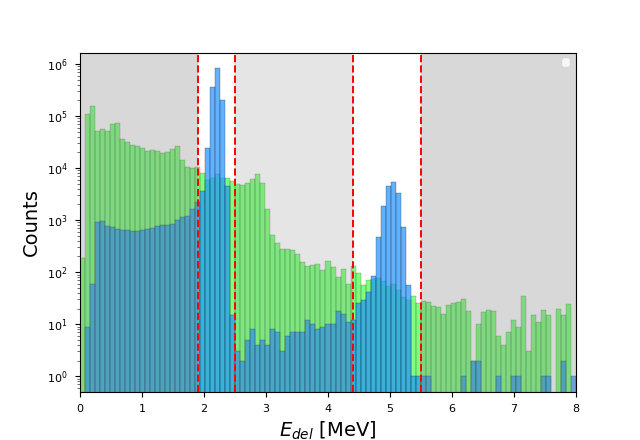
\includegraphics[width=7.5cm]{Images/Cut/e_del.png}
			\label{fig:e_del_cut}
			
		\end{wrapfigure}
		
		\vspace*{0.15cm}
		
		These energy selection windows are aligned with the energies characteristic of neutron capture on hydrogen and carbon atoms. The energy of the delayed signal is a hallmark of the neutron capture process and varies based on the capturing element. The chosen ranges are deliberately selected to coincide with the expected energy signatures for neutron capture on hydrogen and carbon within the detector, which is essential for accurately isolating and analyzing the events of interest.
		\newline
		
	\end{adjustbox}

\end{enumerate}

\vspace{-1cm}

\subsubsection{Results}
The evaluation showcased the algorithm's adeptness in pinpointing true IBD events and distinguishing them from background noise. The findings, encompassing the accuracy for true IBD events and efficiency for background events, are organized in two tables. The confusion matrix (Table \ref{tab:confusion_matrix_cut}) offers a comprehensive classification breakdown, while the summary table (Table \ref{tab:performance_cut}) highlights accuracy rates. The notable efficiency and scarce misclassification of background events underscore the algorithm's prowess in curbing false positives. It is important to highlight that the evaluation was conducted on the test dataset.


\vspace{-0.2 cm}
\begin{figure}[h!]
	\centering
	\small
	\hspace{-4cm}
	\begin{minipage}{0.3\textwidth}
		\begin{tabular}{cc}
			\toprule
			 & \textbf{Manual Cut} \\ 
			\midrule
			\textbf{IBD Efficiency} &  97.702\% \\ 
			\textbf{BKG Efficiency} &  99.997\% \\ 
			\bottomrule
		\end{tabular}
		\captionof{table}{Performance}
		\label{tab:performance_cut}
	\end{minipage}
\hspace{1.5cm}
	\begin{minipage}{0.5\textwidth}
		\centering
		\begin{tabular}{ccc}
			\toprule
			& \textbf{Predicted BKG} & \textbf{Predicted IBD} \\
			\midrule
			\textbf{Actual BKG} & 200640 & 7 \\
			\textbf{Actual IBD} & 4542 & 194844 \\
			\bottomrule
		\end{tabular}
		\captionof{table}{Confusion Matrix}
	\label{tab:confusion_matrix_cut}
	\end{minipage}
	\hspace{-2cm}
\end{figure}

\vspace{-1.5 cm}

\subsection{XGBoost}
XGBoost is a gradient-boosting decision tree algorithm, known for its speed and performance, achieved through parallel processing. It's well-suited for complex patterns, making it ideal for the JUNO experiment's event selection.
The XGBoost model was configured with specific settings and hyperparameters:

\begin{itemize}
	\item  \textbf{Random seed (\texttt{seed})} : Set to 1 for reproducibility, ensuring consistent random number generation.
	\item  \textbf{Number of estimators (\texttt{n\_{estimators}})} : Configured with an initial value of 10,000 decision trees, controlling model complexity. However, during training, the number of estimators was automatically determined using the early stop condition, which monitors the model's performance on a validation set.
	\item  \textbf{Learning rate (\texttt{learning\_rate})} : Set at 0.05, dictating each tree's contribution to the final prediction. 
	\item  \textbf{Maximum tree depth (\texttt{max\_depth})} : Limited to 3, controlling the complexity of each tree.
\end{itemize}
The chosen hyperparameters strike a balance between computational efficiency and model performance, allowing control over the learning process and model complexity. To optimize the XGBoost model, a Grid Search technique was used. This method evaluated various settings and hyperparameter combinations to identify the optimal configuration that maximizes model accuracy.



\subsubsection{Results}
The algorithm exhibited higher efficiency in identifying true IBD events and distinguishing them from background events. A confusion matrix was constructed to provide a comprehensive understanding of the model's precision and effectiveness.

The confusion matrix, presented in Table \ref{tab:conf_matrix_xgb}, reveals the number of true positives, false positives, true negatives, and false negatives. The exceptionally low number of false positives and false negatives underscores the algorithm's effectiveness in minimizing misclassifications.

Additionally, the efficiency rates for IBD and background classifications are summarized in a separate table. The high efficiency rates further emphasize the algorithm's proficiency in both identifying true IBD events and rejecting background events.

To avoid bias from the dataset used for the model evaluation, it's important to note that the evaluation was carried out on the test dataset.

\begin{figure}[h!]
	\centering
	\begin{minipage}{0.33\textwidth}
	\centering
	\begin{tabular}{cc}
		\toprule
		& \textbf{XGBoost} \\
		\midrule
		\textbf{IBD Efficiency} & 99.9985\% \\
		\textbf{BKG Efficiency} & 99.9979\% \\
		\bottomrule
	\end{tabular}
	\captionof{table}{Performance}
	\end{minipage}
	\begin{minipage}{0.65\textwidth}
	\centering
	\begin{tabular}{ccc}
		\toprule
		& \textbf{Predicted IBD} & \textbf{Predicted BKG} \\
		\midrule
		\textbf{Actual IBD} & 199811 & 4 \\
		\textbf{Actual BKG} & 3 & 200215 \\
		\bottomrule
	\end{tabular}
	\captionof{table}{Confusion Matrix}
	\label{tab:conf_matrix_xgb}
\end{minipage}
\end{figure}




\subsubsection{Interpretation of the model}
In our study, we used \textbf{SHAP} (SHapley Additive exPlanations)  \cite{shap}, to interpret the predictions of a trained XGBoost model. SHAP utilizes concepts from game theory, treating predictions as a "game" where features are the "players". The SHAP value for a feature is its average contribution to every possible combination of features.

The shapley value, \(\phi_i\), for feature \(i\) is calculated using:

\begin{equation}
	\phi_j(x) = \sum_{S \subseteq M\setminus\{j\}} \frac{|S|!(M-|S|-1)!}{M!} [f(x_S \cup \{j\}) - f(x_S)]
\end{equation}

Here, \(N\) is the set of all features, \(S\) is a subset of \(N\) excluding feature \(i\), and \(f(S)\) is the model's prediction with feature set \(S\). The term \(|S|!(|M| - |S| - 1)! / |M|!\) assigns a weight to each subset based on the number of times it appears in all permutations of the features.\\



Based on the calculation of SHAP values, we can construct visualizations that aid in analyzing and understanding how the model has learned to differentiate between IBD events and background events. 

\begin{figure}[h!]
	\centering
	\begin{minipage}{0.5\textwidth}
		\centering
		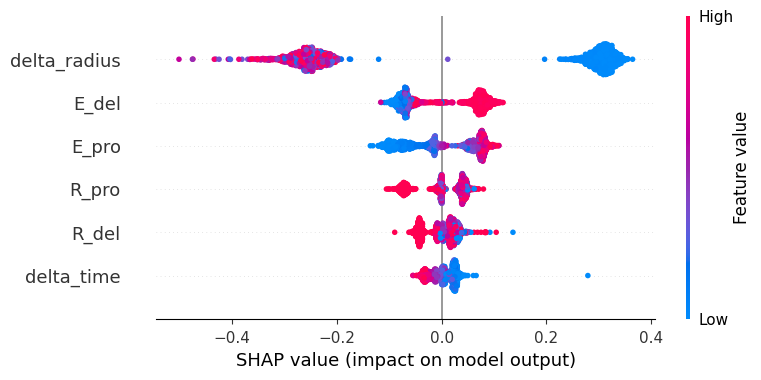
\includegraphics[width=\linewidth]{Images/Shap/summary_plot}
		\caption{XGBoost Summary Plot}
		\label{fig:summary_plot}
	\end{minipage}%
	\begin{minipage}{0.5\textwidth}
		\centering
		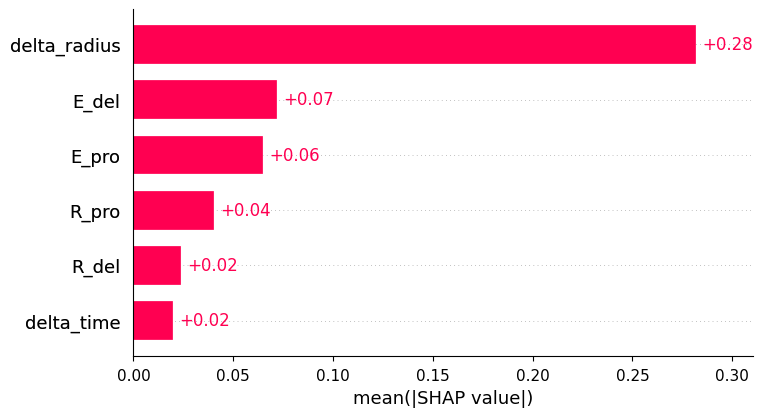
\includegraphics[width=\linewidth]{Images/Shap/feature_importance_bar}
		\caption{XGBoost feature importance}
		\label{fig:feature_importance}
	\end{minipage}
\end{figure}


The presented graphs depict the importance of each feature used by the algorithm for learning, measured by calculating the  SHAP values. On Figure \ref{fig:feature_importance}, the x-axis represents the mean absolute SHAP value for each feature. The first key characteristic of the model is evident here: the  most importance feature in classification is $\Delta R$. Here, the importance of the feature $\Delta R$ is underscored by the fact that it possesses the highest mean absolute SHAP value, which is 0.28. Moreover, referring back to the graphs of Figure \ref{fig:hist_features}, it was already observable that $\Delta R$ is the feature that separates the IBD class most distinctly from the BKG class. %A clear separation is evident from $\approx 2500 mm$ onwards, where BKG events prevail, while IBD events are more prevalent below $\approx 2500 mm$. \\

In the left summary plot of Figure \ref{fig:summary_plot}, the x-axis represents the SHAP value and the y-axis represents the various features. Two distinct data clusters for the \(\Delta R\) feature are strikingly evident. For high values of \(\Delta R\), the algorithm yields a negative SHAP value, which corresponds to the expected classification as background (BKG) events. Conversely, for lower values of \(\Delta R\), the algorithm returns positive SHAP values, indicating events accurately identified as IBD. There is a clear separation between these clusters, demonstrating the algorithm's high confidence in categorizing events based on this feature.

Second in order of importance, with a SHAP value approximately four times smaller than that of $\Delta R$, is $E_{del}$, the energy of the delayed event. Comparing with the feature histogram in Figure \ref{fig:hist_features}, it's clear that, focusing on the $E_{del}$ distribution, most BKG data occupy the initial part of the histogram, thus at lower energies, and the algorithm has learned to determine that for lower delayed signal energies, the event is classified as a BKG event, based on the summary plot and the value of the SHAP value. For slightly higher energies, given the presence of characteristic peaks that significantly increase the counts of IBD events, the algorithm learns to correctly determine an IBD event. 

Exploring in-depth the analysis of $E_{del}$ feature, a plot was created where the x-axis represents individual events, and the y-axis represents the effect that each event had on the $E_{del}$ feature, the $E_{del} eff$, starting from a '\textit{base value} = 0.53' that is the average of the model's predictions across the entire training dataset. It is observed that around the characteristic peaks of neutron capture at approximately $2.2 MeV$ and $4.9 MeV$, the algorithm has successfully learned to distinguish them from background events with high accuracy.

\begin{figure}[h!]
	\centering
	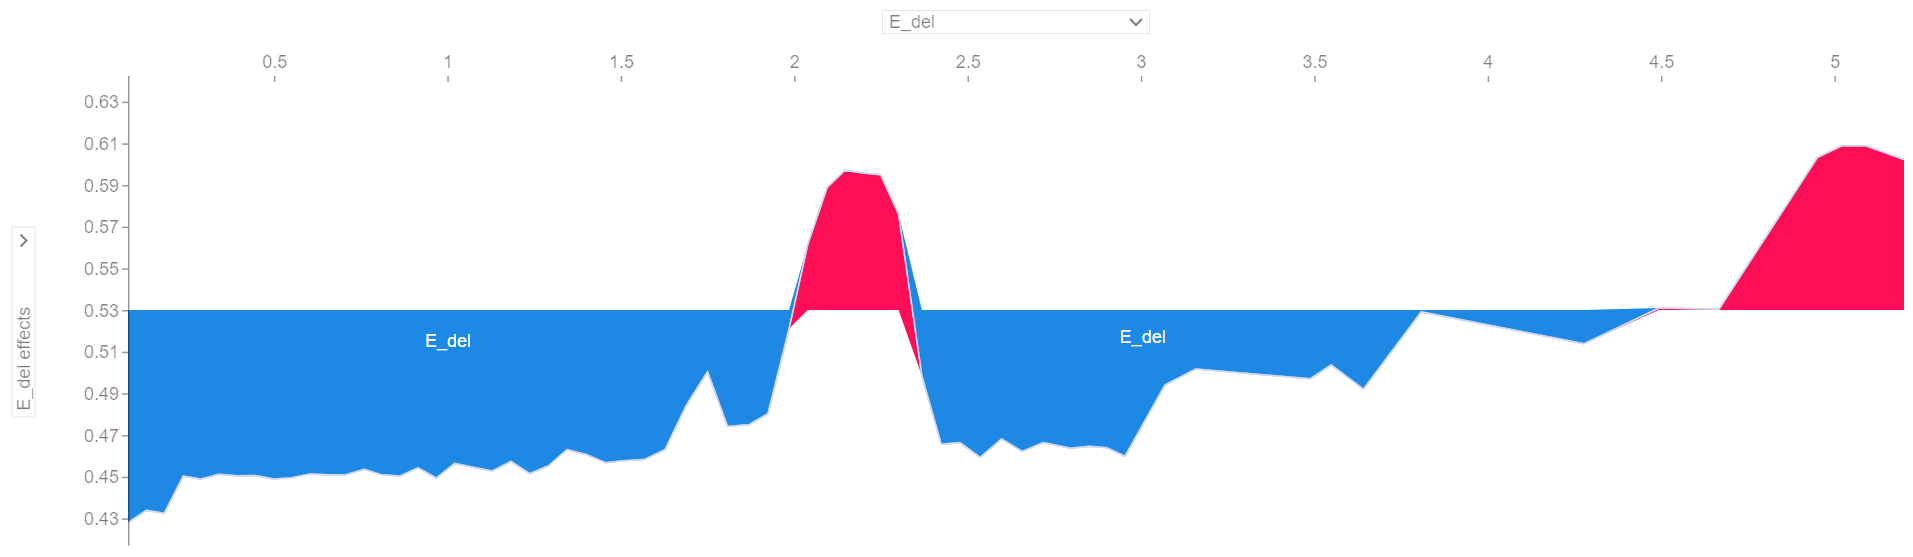
\includegraphics[width=\linewidth]{Images/Shap/E_del_force_plot.png}
	\label{fig:E_del_force_plot}
\end{figure}

Regarding the $E_{pro}$ feature, of Figure \ref{fig:hist_features}, for values below 1 $\si{\mega\electronvolt}$, the histogram is predominantly occupied by BKG events, and as seen from the summary plot (Figure \ref{fig:summary_plot}), these are correctly identified by the algorithm. However, for prompt signals with energies within the positron-like spectrum, the algorithm identifies these events as IBD. The features $R_{pro}$, $R_{del}$, and $\Delta t$ do not contribute as $E_{pro}$, $E_{del}$ and $\Delta R$ to the algorithm's ability to discern between the two classes from their distribution, as there are no clear differences between the feature distribution for IBD and BKG.


Based on the aforementioned information, Figure \ref{fig:waterfall_BKG} and Figure \ref{fig:waterfall_IBD}, show waterfall plots. Two typical events have been chosen, one for IBD and one for BKG.
These plots visually display the individual contributions of each feature to the model's final prediction, which is 1 for IBD events and 0 for background events. The starting point of these plots is the '\textit{base value}', mentioned before. The $f(x)$ shown in the graph represents the predicted value, and is mathematically expressed as:

\begin{equation}
	\text{Final Output} = \text{Base Value} + \sum_{i=1}^{n} \text{SHAP Val}_{i}
\end{equation}

This equation demonstrates how the model arrives at its final prediction by combining the base value with the contributions of each feature through their SHAP values.

\begin{figure}[h!]
	\centering
	\begin{minipage}{0.5\textwidth}
		\centering
		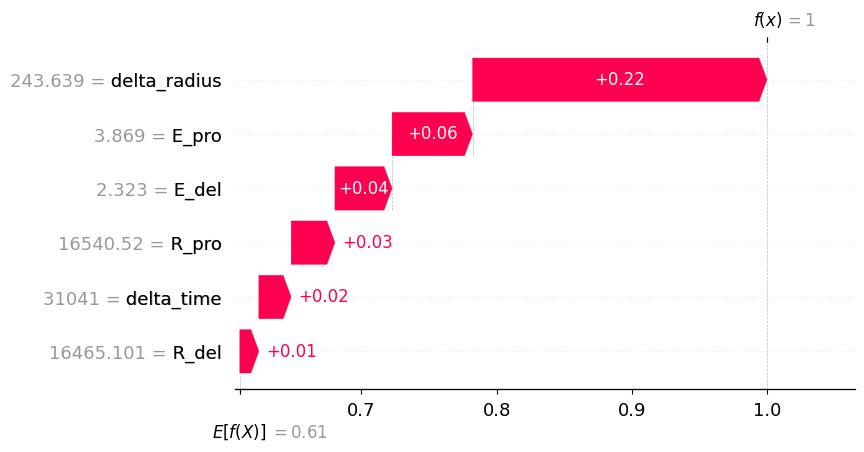
\includegraphics[width=\linewidth]{Images/Shap/waterfall_IBD}
		\caption{Waterfall IBD}
		\label{fig:waterfall_IBD}
	\end{minipage}%
	\begin{minipage}{0.5\textwidth}
		\centering
		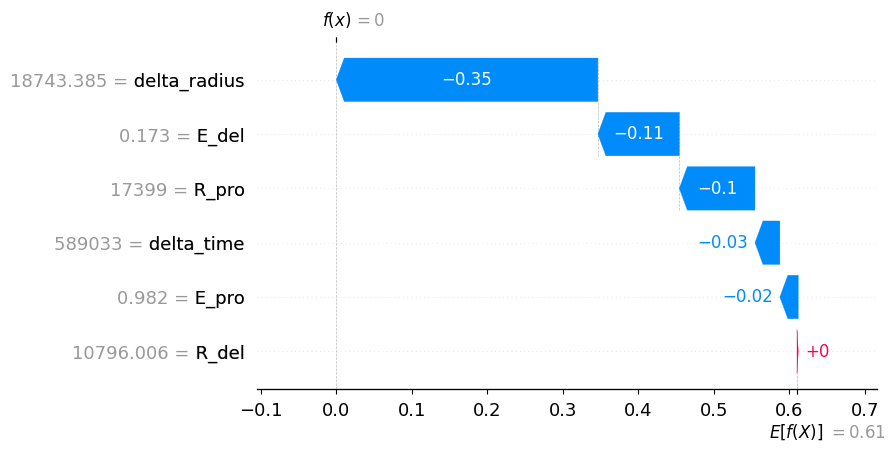
\includegraphics[width=\linewidth]{Images/Shap/waterfall_BKG}
		\caption{Waterfall BKG}
		\label{fig:waterfall_BKG}
	\end{minipage}
\end{figure}

In the SHAP waterfall plots, each feature is represented by a bar, with the length proportional to its SHAP value, indicating its contribution to the prediction. Notably, \texttt{delta\_radius} has the longest bar, reflecting its SHAP value, for both the predictions, indicating that it is the most influential feature in this instance, as we expected. Conversely, \texttt{delta\_time}, \texttt{E\_del}, \texttt{E\_pro} have the shortest bar due to the SHAP value, signifying a lesser contribution of the prediction. This graphical representation provides an intuitive understanding of how each feature is influencing the model's prediction for this particular event, crucial for the interpretability of this models.\\
\newline

It is noteworthy to observe how the SHAP values exert influence on the predictions of two mislabeled events, which are, respectively, \textit{False Positive} (Figure \ref{fig:waterfall_FP}) and \textit{False Negative} (Figure \ref{fig:waterfall_FN}) predictions:


\begin{figure}[h!]
	\centering
	\begin{minipage}{0.5\textwidth}
		\centering
		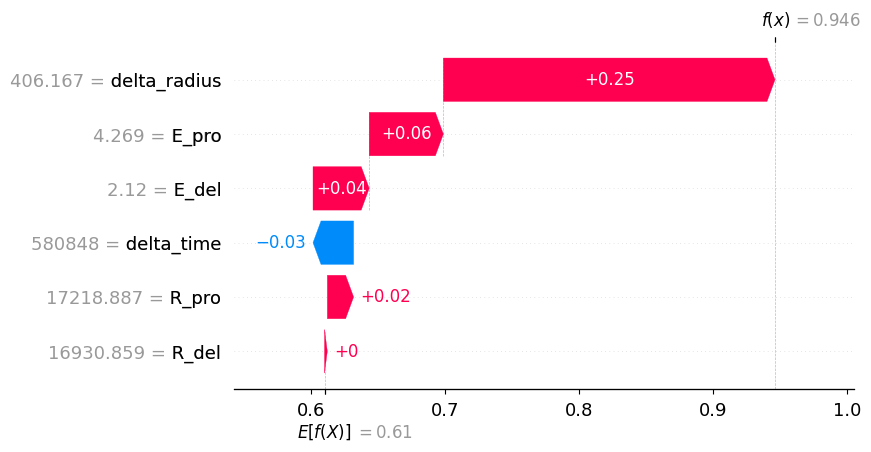
\includegraphics[width=\linewidth]{Images/Shap/waterfall_FP}
		\caption{Waterfall FP}
		\label{fig:waterfall_FP}
	\end{minipage}%
	\begin{minipage}{0.5\textwidth}
		\centering
		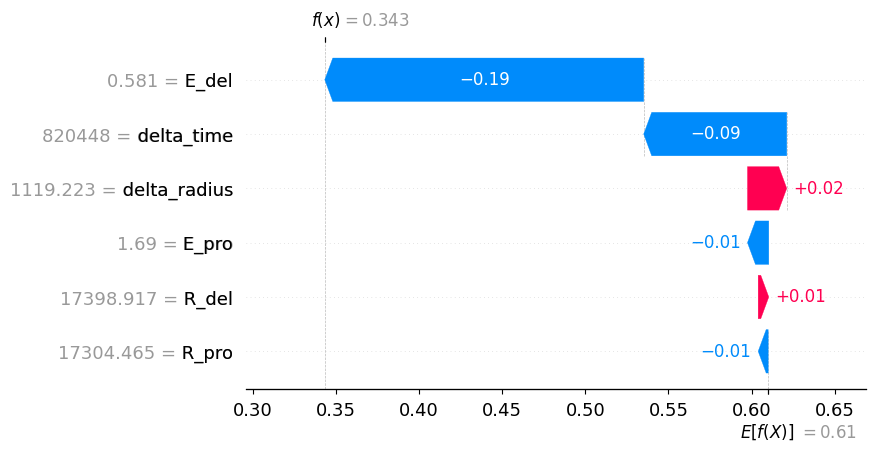
\includegraphics[width=\linewidth]{Images/Shap/waterfall_TN}
		\caption{Waterfall FN}
		\label{fig:waterfall_FN}
	\end{minipage}
\end{figure}


For the \textit{False Negative} case, the most significant feature contributing to the misclassification of the event is $E_{del}$, which is approximately 0.6 MeV. This value does not fall within the characteristic peaks of neutron capture but instead lies in a region where background events are much more probable, as can be compared with Figure \ref{fig:hist_features}. It's important to note that for this particular event, $E_{del}$ is the most influential feature, whereas for most other events, $\Delta R$ (\texttt{delta\_radius}) tends to have a greater contribution. The SHAP value for the $\Delta R$ feature is positive, indicating that this feature suggests the event to be a true IBD, but it is not sufficient for correct labeling. Additionally, the \texttt{delta\_time} feature contributes to the misclassification because the event falls into a region where background events are prevalent. The other features are not decisive in the misclassification as they have very small positive and negative SHAP values and do not significantly contribute to correctly identifying the event.

For the \textit{False Positive} case, the feature that contributes most to the misclassification is $\Delta R$ (\texttt{delta\_radius}). In this case, a coincidence of background events that are very close to each other spatially is misclassified as IBD primarily for this reason, as seen in Figure \ref{fig:waterfall_FP}. Additionally, contributing to the incorrect classification of this event are $E_{del}$ and $E_{pro}$, which have values in regions that are perfectly compatible with the positron spectrum for $E_{pro}$ and compatible with neutron capture for $E_{del}$. Specifically, $E_{del}$ has a value of approximately 2.2 MeV, which is within the expected range for neutron capture.


In conclusion, the SHAP values and the corresponding plots provide a valuable tool for understanding the decision-making process of the model, highlighting the importance of different features in the classification task. 


\subsection{PyThorch}
The ANN, implemented using the PyTorch library, is made of one input layer, four hidden layers, and one output layer. The number of neurons in the input layer is determined based on the number of features used in the training dataset, so the input layer has six input neurons. Each hidden layer contains 64 neurons and utilizes the \textit{Rectified Linear Unit} (ReLU), defined as $ ReLU(x) = \max(0, x) $, as the activation function. It is not defined an explicit activation function in the output layer of the network, opting instead for a direct linear output.

For training the network, it is first instantiated and the computation has been transferred to a CUDA-enabled Graphics Processing Unit (GPU) to leverage hardware acceleration, using a Virtual Machine on CloudVeneto, equipped with \textit{NVIDIA T4 Tensor Core GPU}, thereby enhancing computational efficiency. The \textit{Cross-Entropy} Loss is chosen as the \textit{loss} function. The network's weights are iteratively adjusted through the use of the Adam optimization algorithm.

The training process consists of up to \textit{2000 epochs}; however, an early stopping mechanism is integrated to prevent overfitting and to reduce computational overhead. Early stopping functions as an intelligent termination criterion for the training process of a machine learning model. When the model is being trained on a dataset and ceases to exhibit improvement in its performance on an independent validation set, early stopping intervenes to halt the training. This ensures that the model maintains a robust ability to generalize to unseen data and does not overfit by excessively adapting to the idiosyncrasies of the training dataset. 
Specifically, the training is terminated if the validation loss does not exhibit improvement for a span of 10 consecutive epochs.


\subsubsection{Results}
The model showed remarkable adeptness in accurately classifying true IBD events and segregating them from the background. To obtain a more detailed representation of the model's accuracy and reliability, a confusion matrix was created, and is shown in Table \ref{tab:conf_matrix_nn}. The notably small quantity of incorrectly classified events in both the IBD and BKG datasets reflects the model's success in reducing misclassifications. In addition, a distinct table summarizes the efficiency rates for the classifications of IBD and background events. The high efficiency rates further underscore the model's capability in correctly identifying true IBD incidents and effectively filtering out background noise.

\vspace{-0.2cm}

\begin{figure}[h]
	\centering
	\small
	\hspace{-3cm}
	\begin{minipage}{0.3\textwidth}
		\centering
		\begin{tabular}{cc}
			\toprule
			& \textbf{Neural Network} \\
			\midrule
			\textbf{IBD Efficiency} & 99.9849\% \\
			\textbf{BKG Efficiency} & 99.9770\% \\
			\bottomrule
		\end{tabular}
		\captionof{table}{Performance}
	\end{minipage}
\hspace{2cm}
	\begin{minipage}{0.5\textwidth}
		\centering
		\begin{tabular}{ccc}
			\toprule
			& \textbf{Predicted IBD} & \textbf{Predicted BKG} \\
			\midrule
			\textbf{Actual IBD} & 200231 & 46 \\
			\textbf{Actual BKG} & 30 & 199726 \\
			\bottomrule
		\end{tabular}
		\captionof{table}{Confusion Matrix}
		\label{tab:conf_matrix_nn}
	\end{minipage}
\hspace{-1cm}
\end{figure}
\vspace{-1cm}

\section{Model Comparison}
It is possible to conduct a comparison among the models based on the results presented in Table \ref{tab:confusion_matrix_cut}, Table \ref{tab:conf_matrix_xgb} and Table \ref{tab:conf_matrix_nn}.\\

The \textit{XGBoost} model demonstrated the lowest misclassifications for both IBD and BKG events. It erroneously predicted only 4 IBD events as BKG and 3 BKG events as IBD. This indicates a high degree of model precision, making it particularly reliable for the identification of both IBD and BKG events.

On the other hand, the \textit{Manual Cut} model showed a significantly higher number of IBD mispredictions, misclassifying 4542 IBD events as background. This could suggest that, although the Manual Cut model has high background efficiency, it may not be the most reliable for IBD event identification.
Nonetheless, this model approach ffers effective background rejection at the expense of a slight decrease in efficiency.


The \textit{PyTorch Neural Network}, finally, demonstrated a slightly higher number of BKG mispredictions compared to XGBoost, misclassifying 30 BKG events as IBD. However, it had a very low number of IBD mispredictions, misclassifying only 46 IBD events as BKG.

In summary, although all three models showed high efficiency in detecting BKG events, the XGBoost model stands out as the most accurate and reliable model for the identification of both IBD and BKG events, according to the provided data. This makes it the model of choice based solely on these tables.\\


Comparing the efficiencies of the models, we observe a significant difference between the Manual Cut model and the machine learning models, XGBoost and PyTorch Neural Network.

The Manual Cut model has an IBD efficiency of $97.702\%$, which, while respectable, is markedly lower than the efficiencies achieved by the machine learning models. The XGBoost model achieves an IBD efficiency of $99.9985\%$, and the PyTorch Neural Network reaches $99.9849\%$ - both considerably higher than the Manual Cut model.

This difference in IBD efficiency underscores the transformative impact of machine learning in predictive modelling, showing its superior capacity to identify complex patterns within the data. The background efficiencies of all models are comparable, showing high performance across the board. However, the edge given by machine learning in IBD efficiency demonstrates the powerful advantage of these advanced algorithms.\\

%--------------------------------------------
Having clearly shown that the efficiency of machine learning models outperforms that of the Manual Cut model, it becomes crucial to delve further into an intricate comparison between two standout machine learning models: XGBoost and the Neural Network.
%------------------------------------------



\subsubsection{XGBoost and Neural Network}
To deeply compare the performance of PyTorch and XGBoost, are presented graphs to illustrate how the two algorithms, evaluate the determination of IBD events in comparison to BKG, based on the values of the features $\Delta R$ and $\Delta t$ and $R_{pro}$.
The graphs of Figure \ref{fig:dr_dt_xgboost} and  Figure \ref{fig:dr_dt_pytorch} illustrate how the two algorithms, XGBoost and PyTorch, evaluate the determination of IBD events in comparison to BKG events, based on the values of the features $\Delta R$ and $\Delta t$.\\


\begin{figure}[h!]
	\centering
	\begin{minipage}{0.5\textwidth}
		\centering
		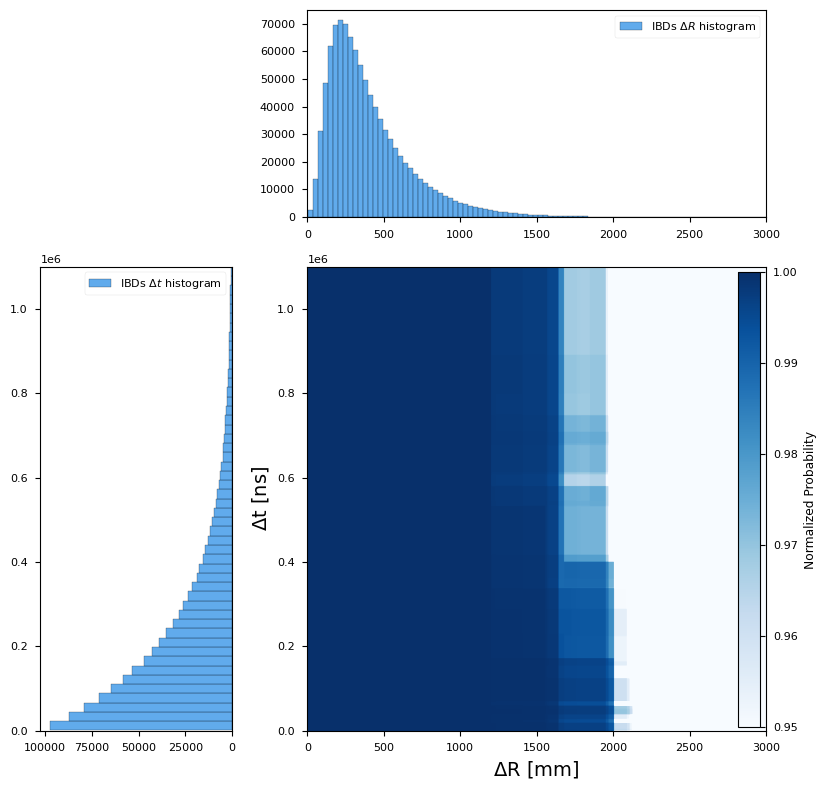
\includegraphics[width=0.9\linewidth]{Images/dr_dt_xgboost}
		\caption{($\Delta R$, $\Delta t$) plot}
		\label{fig:dr_dt_xgboost}
	\end{minipage}%
	\begin{minipage}{0.5\textwidth}
		\centering
		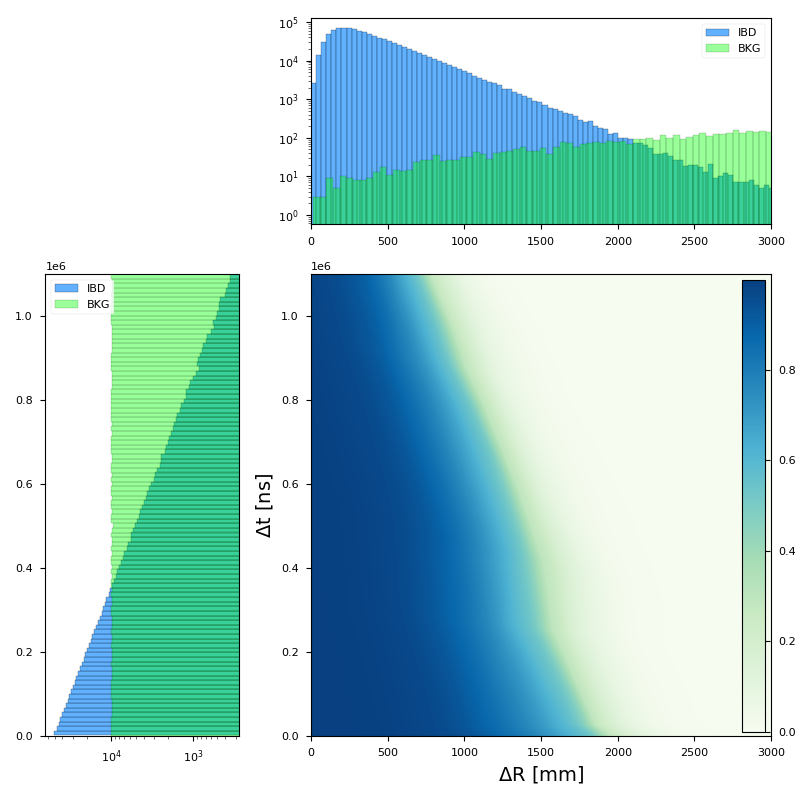
\includegraphics[width=0.9\linewidth]{Images/dr_dt_pytorch}
		\caption{($\Delta R$, $\Delta t$) plot}
		\label{fig:dr_dt_pytorch}
	\end{minipage}
\end{figure}


As expected, by observing the distribution of histograms for IBD events only, it is evident that both algorithms perform accurately for events with $\Delta R$ < 2200mm, where the counts for BKG events begin to surpass the counts of IBD events. The most significant aspect that allows for a comparison between the models through this plot is the feature $\Delta t$. For XGBoost, as shown in the graph, $\Delta t$ does not seem to be very important for determining IBD or BKG events, which is consistent with the feature importance discussed earlier and presented in Figure \ref{fig:feature_importance}. In contrast, for the PyTorch model, the feature $\Delta t$ appears to have notable importance for the accurate identification of events. 
Observing the distribution of the $\Delta t$ feature for IBD events reveals an exponential decay, indicating that many IBD events are expected for very low values of $\Delta t$, and gradually decreasing. Combining this trend with the decrease in $\Delta t$ events, a graph similar to the one presented for PyTorch is expected. Therefore, even though the PyTorch model has lower efficiency, it seems to better evaluate the importance of the $\Delta t$ feature, which is not achieved with the XGBoost algorithm.\\


The graphs in Figure \ref{fig:dr_r_xgboost} and Figure \ref{fig:dr_r_pytorch} demonstrate the evaluation of XGBoost and PyTorch in determining IBD events compared to BKG events, using the feature values of $\Delta R$ and $R_{pro}$.  \\

\vspace{-0.5cm}
\begin{figure}[h!]
	\centering
	\begin{minipage}{0.5\textwidth}
		\centering
		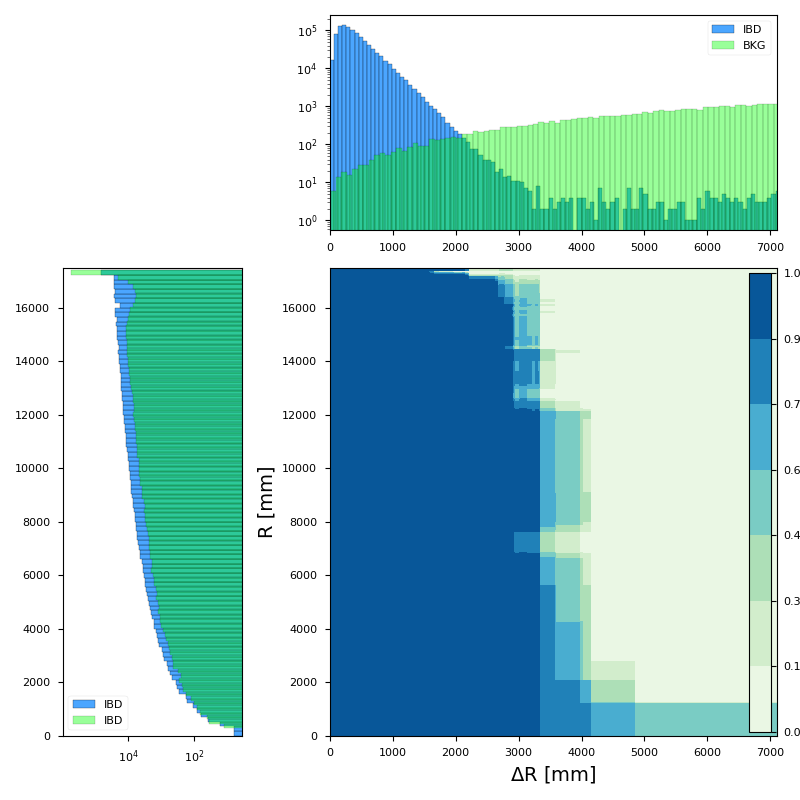
\includegraphics[width=0.9\linewidth]{Images/dr_r_xgboost}
		\caption{($\Delta R$, $R_{pro}$) plot}
		\label{fig:dr_r_xgboost}
	\end{minipage}%
	\begin{minipage}{0.5\textwidth}
		\centering
		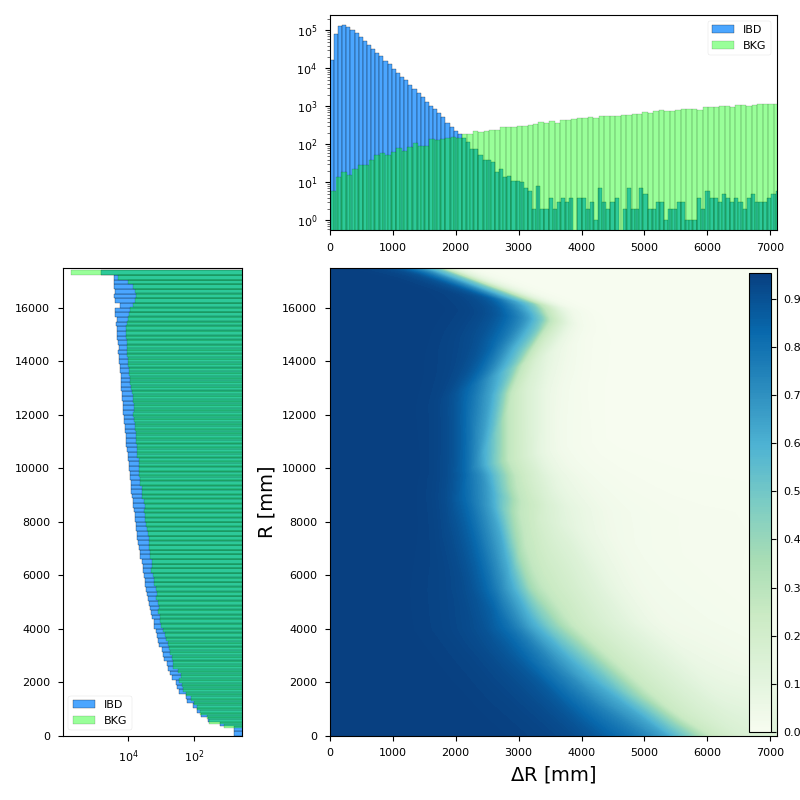
\includegraphics[width=0.9\linewidth]{Images/dr_r_pytorch}
		\caption{($\Delta R$, $R_{pro}$) plot}
		\label{fig:dr_r_pytorch}
	\end{minipage}

\end{figure}



Both algorithms, XGBoost and PyTorch, have effectively learned to distinguish the substantial differences between IBD and BKG events based on these features. Specifically, when approaching the boundary, there is a significant presence of BKG events attributable to various materials such as acrylic, steel bars, the glass of the photomultiplier tubes (PMTs), and radon in the water. More precisely, for $\Delta R > 4000 mm$ in XGBoost and $\Delta R > 5500 mm$ in PyTorch, there is a clear separation between IBD and BKG events.

However, it is important to consider the distribution of $R_{pro}$. As observed during the feature presentation, around $R_{pro} \approx 16000$ mm, there is a drop in the count of background events, followed by a resurgence. 
Interestingly, the ($R_{pro}$, $\Delta R$) PyTorch graph (Figure \ref{fig:dr_r_pytorch}) shows that the neural network has successfully captured and utilized this behaviour to effectively distinguish IBD events that fall within this range.\\


This is evident as a peak in probability in the ($R_{pro}$, $\Delta R$) plot along the $R_{pro}$ axis.
It is important to analyze the behavior of the neural network with respect to the $E_{del}$ and $E_{pro}$ features.
As illustrated in Figure \ref{fig:e_del_e_pro_pytorch}, the Neural Network (NN) encounters challenges in effectively distinguishing Inverse Beta Decay events that occur within the characteristic peaks of $E_{del}$.

\begin{wrapfigure}{t}{0.5\linewidth}
	\caption{($E_{del}, E_{pro}$) PyTorch}
	\vspace{-0.2\baselineskip}
	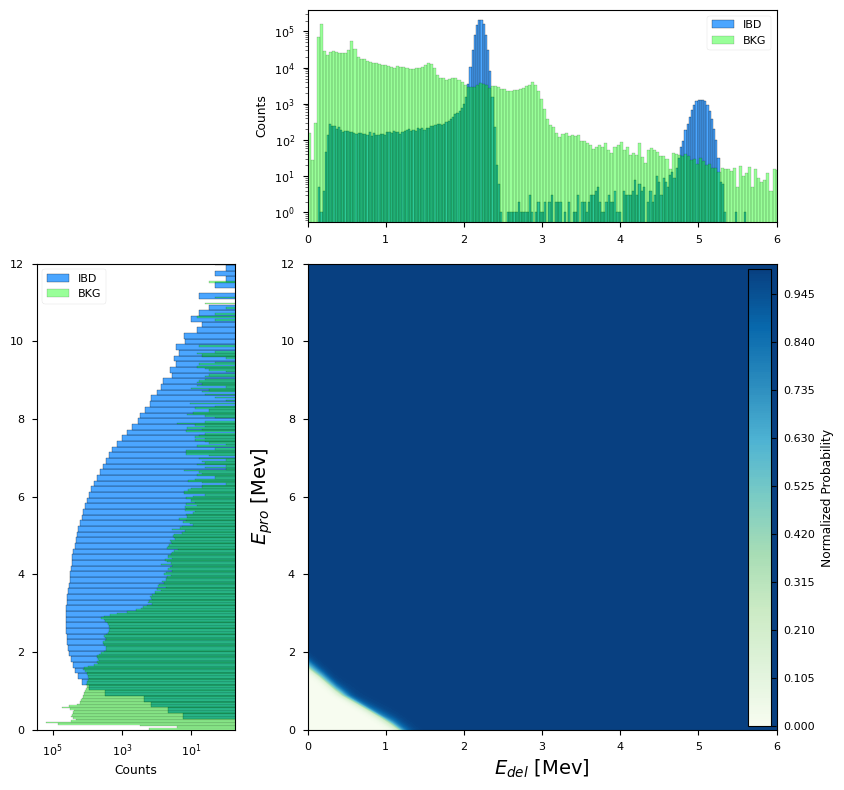
\includegraphics[width=8.5cm]{Images/e_del_e_pro_pytorch}
	\label{fig:e_del_e_pro_pytorch}
	\vspace{-0.5cm}
\end{wrapfigure}


This limitation can be primarily attributed to the insufficient training of the Neural Network (NN), as demonstrated by the observed plot of $E_{pro}$ and $E_{del}$ and the subsequent outcomes, which clearly demonstrate a notable discrepancy when compared to the performance achieved by the Manual Cut approach. The precise reasons for this inadequacy remain uncertain, and it is plausible that a combination of factors contributes to this phenomenon. Potential factors may comprise various training constraints, or challenges in optimizing the network's hyperparameters. Additionally, the simplistic architecture of the NN, with limited layer. Furthermore, the presence of outliers within the energy values used for training, along with subsequent scaling operations, might introduce further complexities and adversely affect the NN's discriminative capabilities. A comprehensive analysis of these factors, accompanied by rigorous experimentation and fine-tuning, is necessary to elucidate the underlying causes and devise potential solutions for enhancing the NN's performance in this context.
 
\subsubsection{Efficiency and purity}
To better evaluate the models' selection capabilities, the selection efficiency and purity are calculated based on the number of events per day from source neutrinos, \textit{Accidental Background}, and \textit{Correlated Background}. These calculations involve a combination of factors, including Event/Day and a muon cut, applied to a variety of event types. These include Reactor events, our primary source of antineutrinos, and Correlated Background events, such as Geo-U, Geo-Th, Li9, He8, World Reactors, Atmospheric Neutrinos, Fast Neutrons, and $\mathrm{C}$($\alpha,n)$$^{16}\mathrm{O}$. The results are presented to in Table \ref{tab:correlated}. The expected IBD events from Accidental background are also evaluated, as detailed in Table \ref{tab:accidentals}.

For each event type, the selection efficiency for IBD (shown in Tables \ref{tab:confusion_matrix_cut}, \ref{tab:conf_matrix_xgb}, and \ref{tab:conf_matrix_nn}) is multiplied by the \texttt{muon cut} and the events per day to derive the number of IBD events expected when applying the model to the true events generated each day. The calculation for expected IBD events from Accidentals is performed also by multiplying the \texttt{muon cut}, the events per day, and the background efficiency reported in the table, minus 1.

\begin{table}[h]
	\centering
        \small
	\begin{tabular}{lcc|ccc}
		\toprule
		& \textbf{ev/day} & \textbf{muon cut} & \textbf{Manual Cut} & \textbf{XGBoost} & \textbf{PyTorch} \\
		\midrule
		\textbf{Reactor} & 57.4 & 0.916 & 51.4 & 52.6 & 52.6 \\
		\midrule
		\textbf{Geo-U} & 1.155 & 0.916 & 1.03 & 1.06 & 1.06 \\
		\textbf{Geo-Th} & 0.345 & 0.916 & 0.31 & 0.32 & 0.32 \\
		\textbf{Li9} & 0.81 & 1 & 0.79 & 0.81 & 0.81 \\
		\textbf{He8} & 0.09 & 1 & 0.09 & 0.09 & 0.09 \\
		\textbf{World Reactors} & 1.22 & 0.916 & 1.09 & 1.12 & 1.12 \\
		\textbf{Atmospheric $\nu$} & 0.2 & 0.916 & 0.18 & 0.18 & 0.18 \\
		\textbf{Fast neutron} & 0.12 & 0.916 & 0.11 & 0.11 & 0.11 \\
		\textbf{$\mathrm{C}$($\alpha,n)$$^{16}\mathrm{O}$} & 0.06 & 0.916 & 0.05 & 0.05 & 0.05 \\
		\textbf{Total} & -- & -- & 55.02 & 56.32 & 56.31 \\
		\bottomrule
	\end{tabular}
	\caption{IBD expected from \textit{Reactors} and \textit{Correlated Background}}
	\label{tab:correlated}
\end{table}

\begin{table}[h]
	\centering
        \small
	\begin{tabular}{lcc|ccc}
		\toprule
		& \textbf{ev/day} & \textbf{muon cut} & \textbf{Manual Cut} & \textbf{XGBoost} & \textbf{PyTorch} \\
		\midrule
		\textbf{Accidentals} & 134124.0 & 0.916 & 22.69 & 18.22 & 209.01 \\
		\bottomrule
	\end{tabular}
	\caption{IBD expected from \textit{Accidental Background}}
	\label{tab:accidentals}
\end{table}
	

Finally, the efficiency and purity were calculated as the number of selected IBDs divided by the overall IBDs and the number of selected IBDs divided by the total selected events, respectively. This method provides an estimation of the selection algorithm's efficiency and purity, reported in Table \ref{tab:eff_pur}.

\begin{table}[htp]
	\centering
	\small
	\begin{tabular}{lccc}
		\toprule
		& \textbf{Manual Cut} & \textbf{XGBoost} & \textbf{Neural Network} \\
		\midrule
		\textbf{Purity} & 0.6610 & 0.7054 & 0.1981 \\
		\textbf{Efficiency} & 0.8949 & 0.9160 & 0.9158 \\
		\bottomrule
	\end{tabular}
	\caption{Performance Evaluation}
	\label{tab:eff_pur}
\end{table}











